\problemWithTimeMem{让火焰净化一切!}{1 second}{1024MB}

Rhyme和Arthas又在偷偷摸鱼,开启了一局紧张刺激的炉石传说标准对战。

“让火焰净化一切!”Rhyme拍下了炎魔之王拉格纳罗斯,这张久负盛名的中立传说卡牌,江湖人称大螺丝。他的效果是:“无法攻击。在你的回合结束时,随机对一个敌人造成 $8$ 点伤害。”这天的天气如此燥热,大螺丝的效果得到了极大的提升乃至影响了游戏的平衡。此时双方无法进行任何操作,只剩下大螺丝在每回合结束时肆意的向对方某一目标释放一个高达 $8$ 点伤害的火球。

现在,Arthas本身只剩 $x$ 滴血,他的场上只有一个 $y$ 血的随从。当随从的血量降到 $0$ 及以下,随从会从场上消失,\textbf{不会再成为大螺丝的火球目标};当Arthas的血量降到 $0$ 及以下,大螺丝宣告\textbf{游戏结束}。在这个稳赢的局面下,大螺丝想知道它需要\textbf{多少回合的期望}才能终结这场游戏。不过大螺丝不太擅长计算,它将这个任务交给了将它从黑石山召唤出来的Rhyme。

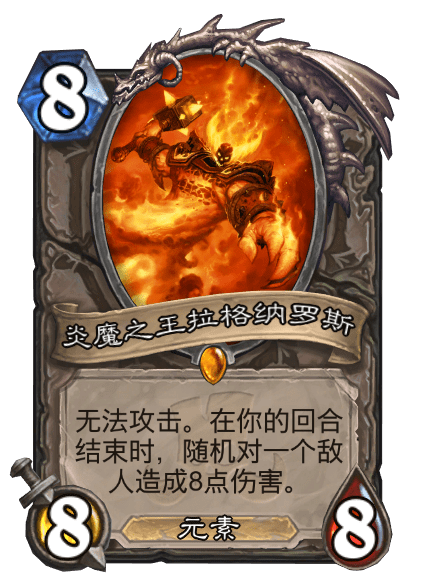
\includegraphics[width=.3\linewidth]{image3.png}


\sout{~~“装配,行动,完美。” 当然,大螺丝并没有这么强力,它既没能斩杀对手,也没能活到游戏最后。这}

\sout{一切只是它被Arthas下回合拍下的新版奇利亚斯一脚送走之前的幻想罢了。~~}

\mysec{Input}

第一行一个整数 $T$,代表共 $T$ 组数据。($1 \leqslant T \leqslant 50$)

此后共 $T$ 行,每行包含两个正整数 $x$ 和 $y$ ,分别代表Arthas本身及其随从的血量 $x$ 和 $y$ 。($1 \leqslant x, y \leqslant 40000$)

额外的,$T$ 组数据中 $x$ 的总和与 $y$ 的总和均不超过 $40000$。


\mysec{Output}

每行一个答案,代表大螺丝消灭对方英雄的回合数期望(误差不超过$10^{-6}$)。

\ACMIO{Sample 1}{%
2

2 3

16 9
}{%
1.500000

3.250000
}

\mysec{Hint}

第一组数据中,$x$ 和 $y$ 最初分别为 $2$ 和 $3$ ,可能出现如下情况:

第一回合攻击Arthas,$x = 2 - 8 = -6 \leqslant 0$,游戏结束,总回合数为 $1$;

第一回合攻击随从,$y = 3 - 8 = -5 \leqslant 0$,随从退场,第二回合攻击Arthas,$x = 2 - 8 = -6 \leqslant 0$,游戏结束,总回合数为 $2$。

答案为:$1 \times \frac{1}{2} + 2 \times \frac{1}{2} = 1.500000$。

第二组数据中,$x$ 和 $y$ 最初分别为 $16$ 和 $9$,答案为:$2 \times \frac{1}{4} + 3 \times \frac{1}{4} + 4 \times \frac{1}{2} = 3.250000$。
